\documentclass[12pt,a4paper,bibliography=totocnumbered,listof=totocnumbered]{article}
% u.U. muss Koma-Skript Package ueber MikTeX deinstalliert und neu installiert werden
% Hilft das nicht, so sollte statt scrartcl die Dokumentenklasse article verwendet werden
\usepackage[backend=bibtex,style=alphabetic]{biblatex}
\usepackage[ngerman]{babel}
\usepackage[utf8]{inputenc}
\usepackage{csquotes}
\usepackage{ifthen}
\usepackage{xargs}
\usepackage{amsmath}
\usepackage{nccmath, mathtools}
\usepackage{amsfonts}
\usepackage{amssymb}
\usepackage{graphicx}
\usepackage{fancyhdr}
\usepackage{tabularx}
\usepackage{geometry}
\usepackage{multirow}
\usepackage{threeparttable}
\usepackage{xurl}
\usepackage{longtable}
\usepackage{makecell}
\usepackage{setspace}
\usepackage[right]{eurosym}
\usepackage[printonlyused]{acronym}
\usepackage{subfig}
\usepackage{floatflt}
\usepackage{float}
\usepackage[usenames,dvipsnames]{color}
\usepackage{colortbl}
\usepackage{paralist}
\usepackage{array}
\usepackage{parskip}
\usepackage[right]{eurosym}
\usepackage[subfigure,titles]{tocloft}
\usepackage[pdfpagelabels=true]{hyperref}
% added includes
\usepackage{tikz}
\usetikzlibrary{matrix,chains,positioning,decorations.pathreplacing,arrows}
\usepackage{pgfplots}
\usepackage{wrapfig}
\usepackage{listings}

\lstset{basicstyle=\footnotesize, captionpos=b, breaklines=true, showstringspaces=false, tabsize=2, frame=lines, numbers=left, numberstyle=\tiny, xleftmargin=2em, framexleftmargin=2em}
\makeatletter
\def\l@lstlisting#1#2{\@dottedtocline{1}{0em}{1em}{\hspace{1,5em} Lst. #1}{#2}}
\makeatother

\geometry{a4paper, top=27mm, left=20mm, right=20mm, bottom=35mm, headsep=10mm, footskip=12mm}

\definecolor{javared}{rgb}{0.6,0,0} % for strings
\definecolor{javagreen}{rgb}{0.25,0.5,0.35} % comments
\definecolor{javapurple}{rgb}{0.5,0,0.35} % keywords
\definecolor{javadocblue}{rgb}{0.25,0.35,0.75} % javadoc
\definecolor{gray}{rgb}{0.6,0.6,0.6}
 
\lstset{language=Java,
basicstyle=\ttfamily\footnotesize,
keywordstyle=\color{javapurple}\bfseries,
stringstyle=\color{javared},
commentstyle=\color{javagreen}\itshape\bfseries,
morecomment=[s][\color{javadocblue}]{/**}{*/},
numbers=left,
numberstyle=\tiny\color{gray},
stepnumber=1,
numbersep=10pt,
tabsize=3,
showspaces=false,
showstringspaces=false}
% Kopf- und Fusszeile
\renewcommand{\sectionmark}[1]{\markright{#1}}
\renewcommand{\leftmark}{\rightmark}
\pagestyle{fancy}
\lhead{}
\chead{}
\rhead{\thesection\space\contentsname}
\lfoot{}
\cfoot{}
\rfoot{\ \linebreak Page \thepage}
\renewcommand{\headrulewidth}{0.4pt}
\renewcommand{\footrulewidth}{0.4pt}

% Vorspann
\renewcommand{\thesection}{\Roman{section}}
\renewcommand{\theHsection}{\Roman{section}}
\pagenumbering{Roman}

\newcommand{\folgen}[1]{
\ensuremath
#1
}

\newcommandx{\student}[4][]{
	\def\studentName{#1}%
	\def\studentMatnr{#2}%
	\def\studentStudiengang{#3}%
	%\def\studentEmail{#4}%
}

\newcommandx{\MyTitelseite}[8][]{
\thispagestyle{empty}

\includegraphics[scale=0.2]{pics/oth-logo.png}\hfill\includegraphics[scale=0.5]{#1}
\begin{center}
\ifthenelse{\equal{#2}{2}}{ % then
	\vspace*{2cm}
	\Large
	\textbf{Ostbayerische Technische Hochschule Regensburg}\\
	\textbf{Fakultät für Informatik und Mathematik}\\
	\vspace*{2cm}
	\Huge
	\textbf{#3}\\[1em]
	\large
	GenerationColorPrint AG\\
	\vspace*{1cm}
	\Large
	\textbf{#4}\\
}{ % else
	\vspace*{1cm}
	\Large
	\textbf{#4}\\
	\vspace*{2cm}
	\large
	An der Fakultät für Informatik und Mathematik der\\
	Ostbayerischen Technischen Hochschule Regensburg\\
	im Studiengang\\
	\studentStudiengang\\[2em]
	eingereichte\\
	\vspace*{1cm}
	\Large
	\textbf{#3}\\[2em]
	\large
	zur Erlangung des akademischen Grades des\\
	\ifthenelse{\equal{#3}{Bachelorarbeit}}{Bachelor of Science (B.Sc.)}{Master of Science (M.Sc.)}
	\vspace*{1cm}
	\Large
}
	\vfill
	\normalsize
	\newcolumntype{x}[1]{>{\raggedleft\arraybackslash\hspace{0pt}}p{#1}}
	\begin{tabular}{rl}%{6cm}p{7.5cm}}
		\rule{0mm}{1ex}\textbf{Vorgelegt von:} & \studentName \\
		%\rule{0mm}{1ex}\textbf{E-Mail:} & \studentEmail \\
		\rule{0mm}{1ex}\textbf{Matrikelnummer:} & \hspace*{-0.5em}\begin{tabular}[t]{r}\studentMatnr\end{tabular} \\ 
		\ifthenelse{\equal{#2}{1}}{~\\}{\rule{0mm}{1ex}\textbf{Studiengang:} & \studentStudiengang \\[2em]}
		\rule{0mm}{1ex}\textbf{Erstgutachter:} & #5 \\ 
		%\rule{0mm}{1ex}\textbf{Team:} & #6 \\[2em]
		\rule{0mm}{1ex}\textbf{Abgabedatum:} & #6 \\ 
	\end{tabular} 
\end{center}
\pagebreak
}
\addbibresource{literature.bib}

\begin{document}


% ----------------------------------------------------------------------------------------------------------
% Cover page
% ----------------------------------------------------------------------------------------------------------
\newcommand{\studierenderName}{Tianhua Dai}
\student{\studierenderName}		% Student's Name
{Matriknummer}						% Student Number
{Wirtschaftsinformatik}			% Study Programme
{tianhua.dai@st.oth-regensburg.de}	% Student's Email

\MyTitelseite{pics/leer}	% Optionally Logo of Supervising Company
{2}								% Style of Cover Page (1 or 2)
{Typ der Arbeit}				% Type of thesis (\in {Bachelor Thesis, Master Thesis})
{Titel}				% Title of Thesis					
{Dr.\ Max Mustermann}		% Primary Supervising Professor
%{Teilnehmer}	% Team members
{05.06.2020}				% Submission Date
\pagebreak

%\setcounter{page}{1} 

% ----------------------------------------------------------------------------------------------------------
% Table of Contents
% ----------------------------------------------------------------------------------------------------------
\setcounter{tocdepth}{2}
\tableofcontents
\pagebreak

% ----------------------------------------------------------------------------------------------------------
% Content
% ----------------------------------------------------------------------------------------------------------
% Spacing for Headlines

% Header
\renewcommand{\sectionmark}[1]{\markright{#1}}
\renewcommand{\subsectionmark}[1]{}
\renewcommand{\subsubsectionmark}[1]{}
\lhead{Chapter \thesection}
\rhead{\rightmark}

%\onehalfspacing
\setstretch{1.15}
\renewcommand{\thesection}{\arabic{section}}
\renewcommand{\theHsection}{\arabic{section}}
\setcounter{section}{0}
\pagenumbering{arabic}
\setcounter{page}{1}

% ----------------------------------------------------------------------------------
% Chapter: Methodische Grundlagen
% ----------------------------------------------------------------------------------
\section{Methodische Grundlagen}
In diesem Kapitel werden erst die methodischen Grundlagen im Zusammenhang mit DCF-Verfahren erklärt. 
Es bezieht sich um die Vorstellung der Kennzahlen sowohl auch die Grundsätze der Kapitalwertrechnung, dadurch das Verständnis in die praktischen Kapitel tiefer eingegangen werden kann.
\subsection{Ertragswert}
Generell ist der Ertragswert das Ergebnis eines Planungs- und Prognoseproblems:
\[EW = \underset{j}{\max}\sum_{t=1}^{T}\sum_{i=1}^{I}(p_{i} \cdot {CF_{ij}}^{t} \cdot (\frac{1}{1+r})^{t}) \] \\
mit
\begin{align*}
	&\text{j=1, ..., J} &&\text{Strategiealternativen} \\
	&\text{i=1, ..., I} &&\text{Zustandsalternativen, Eintrittswahrscheinlichkeit \(p_{i}\)} \\
	&\text{t=1, ..., T} &&\text{Perioden des Betrachtungszeitraums} \\
	&{CF_{ij}}^{t}  &&\text{finanzieller Überschuss in Periode t bei Zustand i und Strategie j} \\
	&p_{i}  &&\text{Eintrittswahrscheinlichkeit für Zustand i} \\
	&\text{r} &&\text{Kapitalisierungszinsfuß} 
\end{align*}
DCF-Verfahren ist ein sogenannt ertragswertorientiertes Verfahren, bei dem eine Überschussgröße mit Opportunitätszins oder Kapitalkosten auf ihren Gegenwartswert diskontiert wird.
\footnote[1]{\cite{Behringer2009}, S. 101}
\newline
\pagebreak

% ----------------------------------------------------------------------------------
% Chapter: 
% ----------------------------------------------------------------------------------
\section{Vier Methoden des DCF-Verfahrens}
Es wird dazu angegeben, dass unter dem Begriff DCF-Verfahren 4 verschiedene Varianten zu unterscheiden sind. 
Die werden in der folgenden Abbildung dargestellt (siehe Abbildung \ref{fig:dcf} \footnote[2]{\cite{Ballwieser2016}, S. 137}):  \\
\begin{minipage}{\linewidth}
	\centering
	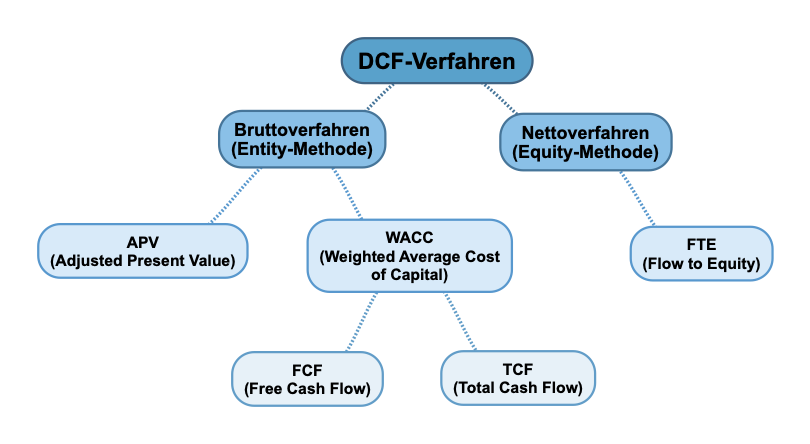
\includegraphics[width=0.5\linewidth]{pics/DCF-Verfahren.png}
	\captionof{figure}[Abbildung 01]{DCF-Varianten}
	\label{fig:dcf}
\end{minipage}	

Dabei wird erst Netto- und Brutto-Ansätze (bzw. Equity- und Entity-Ansätze) unterscheidet. 
Bei den Bruttoverfahren wird der Gesamtwert von Eigenkapital sowie Fremdkapital ermittelt. Und hingegen ist der Wert des Eigenkapitals beim Nettoverfahren erkennbar.
Weiterhin gehört das Flow-to-Equity-Verfahren (FTE) zu Nettoverfahren, und gegenüber steht Bruttoverfahren mit Adjusted-Present-Value-Verfahren (APV) und dem Ansatz für gewogene durchschnittliche Kapitalkosten (WACC).
Zusätzlich gibt es unter dem WACC-Ansatz das Free-Cash-Flow-Verfahren (FCF) und das Total-Cash-Flow-Verfahren (TCF).
\footnote[3]{\cite{Ballwieser2016}, S. 137-138}	\\
Obwohl die obigen Beiden WACC-Ansatz sind, unterscheiden die sich zudem anhand der Berücksichtigung der verschiedenen Steuerzahlungen. Beim FCF-Ansatz geht es um die falschen Steuerzahlungen, dass die Abzugsfähigkeit der Fremdkapitalkosten von den Steuerbemessungsgrundlagen sowie daraus entstehender Steuerprofit nicht berücksichtigt werden. 
Dagegen ist das TCF-Verfahren bei der Cash-Flow-Ermittlung im Zusammenhang mit den richtigen Steuern.
Darüber hinaus basiert der APV-Ansatz auf die Ermittlung von Cash Flow aus einem erdachteten Unternehmen, welches sich rein selbst finanzieren kann. 
Daher wird Free Cash Flow mit eines risikoangepassten Anspruches der Eigentümerrendite diskontiert, statt WACC.
\footnote[4]{\cite{Ballwieser2016}, S. 138-139}	\\
Im Allgemeinen unterscheidet man zwischen der Unternehmenswertermittlung bei einer autonomen Finanzierungspolitik mit proportionaler Ertragsteuer und der Unternehmenswertermittlung bei einer autonomen Finanzierungspolitik in einem Abgeltungssteuersystem. 
Die folgenden Kapiteln werden dann die Arbeitsweise über die 4 Unterarten der DCF-Verfahren sowohl auch ihre Beispielrechnung aufgebaut. 
Dabei wird die Berechnung des Unternehmenswertes mit proportionaler Ertragsteuer durchgeführt.
\pagebreak 

% ----------------------------------------------------------------------------------------------------------
% Filter fuer Literatur und Quellen definieren
% ----------------------------------------------------------------------------------------------------------

\defbibheading{Literatur}{\section*{Literaturverzeichnis}} 
\defbibheading{Quellen}{\section*{Quellenverzeichnis}} 
  
\defbibfilter{Literatur}{\not\keyword{online}} 
\defbibfilter{Quellen}{\keyword{online}} 


% ----------------------------------------------------------------------------------------------------------
% Literatur
% ----------------------------------------------------------------------------------------------------------
\lhead{} 
\rhead{Literaturverzeichnis} 

\printbibliography[heading=Literatur,filter=Literatur] 

\pagebreak


% ---------------------------------------------------------------------------------------------------------- 
% Quellen 
% ---------------------------------------------------------------------------------------------------------- 
\lhead{} 
\rhead{Quellenverzeichnis} 

\printbibliography[title = {Quellenverzeichnis}, heading=Quellen,filter=Quellen] 

\pagebreak 

\end{document}
